\documentclass[12pt,a4paper]{article}

% Margins.
\setlength{\oddsidemargin}{0in}
\setlength{\evensidemargin}{0in}
\setlength{\headheight}{12pt}
\setlength{\headsep}{42pt}
\setlength{\topmargin}{-60pt}
\setlength{\textwidth}{6.5in}
\setlength{\textheight}{10in}
\pagestyle{empty}

\usepackage{amsmath}
\usepackage{float}
\usepackage{graphicx}
\usepackage[hyphens]{url}
\usepackage[hidelinks]{hyperref}	% Clickable links to figures, references and urls.
\usepackage{lastpage}

% Drawing.
\usepackage{pgf}
\usepackage{tikz}

% Listings for formatting code.
\usepackage{listings}
\usepackage{textcomp}
% General options.
\lstset{breaklines=true, basicstyle=\footnotesize\ttfamily, tabsize=4, numbers=none, stepnumber=1, frame=single, showstringspaces=false, upquote=true}
% C++ specific high-lighting. Comments are 50/50 shades of green/black and strings coloured with 60/40 red/black mixture.
\lstset{language=[ISO]C++, commentstyle=\color{green!50!black}, keywordstyle=\color{blue}, stringstyle=\color{red!60!black}}

% Marks of each question.
\def\QOne{10}
\def\Qtwo{10}
\def\Qthree{10}
\def\Qfour{10}
\def\Qfive{10}
\def\Qsix{10}
\def\Qseven{10}
\def\Qeight{10}
\def\Qnine{10}
\def\Qten{10}
\def\TotalMarks{100}

\begin{document}
\begin{minipage}{0.55\textwidth}
{\LARGE \textbf{Physics for Engineers}}\\[0.15cm]
{\normalsize \textbf{Spring 2014 Semester}}\\
{\Large \textbf{Final Exam}}\\
{\normalsize \textbf{Saturday, May 17, 2014}}\\[0.30cm]
{\Large \textbf{Total Time: 180 minutes}}\\[0.15cm]
{\Large \textbf{Total Marks: 100}}\\
\textbf{Course Instructors:}\\
Attique Dawood\\
\end{minipage}
\begin{minipage}{0.4\textwidth}
\textbf{Serial} \hrulefill \\[0.25cm]
\textbf{Name} \hrulefill\\[0.25cm]
\textbf{Section} \rule{1cm}{0.2mm} \textbf{Roll No:} \hrulefill\\[0.25cm]
\textbf{Signature:} \hrulefill\\[0.25cm]
\rule{6.6cm}{0.2mm}\\
\textbf{Signature of Invigilator}\\[0.25cm]
\end{minipage}
\begin{table}[H]
\begin{center}
\vspace{0.3cm}
	{\large \begin{tabular}{|l|c|c|c|c|c|c|c|c|c|c|c|}
	\hline
		\rule{0pt}{2.6ex} Question & \textbf{1} & \textbf{2} & \textbf{3} & \textbf{4} & \textbf{5} & \textbf{6} & \textbf{7} & \textbf{8} & \textbf{9} & \textbf{10} & \textbf{Total}\\
		\hline
		Total Marks \rule{0pt}{2.6ex} & \QOne & \Qtwo & \Qthree & \Qfour & \Qfive & \Qsix & \Qseven & \Qeight & \Qnine & \Qten & \TotalMarks\\
		\hline
		Marks Obtained \rule{0pt}{2.6ex} & & & & & & & & & & &\\
	\hline
	\end{tabular}}
\end{center}
\end{table}
\noindent \textbf{You are advised to READ these notes:}
\begin{enumerate}
\item \textbf{Attempt on the Question Paper. \underline{NO EXTRA SHEET} will be provided/accepted. No
additional sheet will be provided for rough work. Use the back of the page where
provided space is not sufficient.}
\item After asked to commence the exam, please verify that you have \textbf{\pageref{LastPage} different
printed pages} including this title page.
\item There are 10 questions. Attempt all of them. It is advisable to go through the paper once
before starting with the first question.
\item Exam is closed books, closed notes. Please see that the area in your threshold is clean.
You will be charged for any material which can be classified as \textbf{`helping in the paper'}
found near you.
\item All distances and coordinates are in meters.
\item \textbf{Calculator sharing is strictly prohibited.}
\item Students who attempt the paper with lead pencils lose the right to get them rechecked.
\item \textbf{The invigilator present is not supposed to answer any questions. No one may come
to your room for corrections and you are not supposed to request to call anyone.
Make assumptions wherever required and clearly mark them.}
\end{enumerate}
\newpage
\noindent\textbf{Question 1: Line Integral\hfill \QOne~marks}\\
Given a vector field $\textbf{A}=3\rho\hat\rho+\rho^2\phi\hat\phi-3z\hat z$ find the circulation of \textbf{A} ($\oint\limits_{L} \textbf{A}\cdot d\textbf{\textit{l}}$) over the circle of radius $2$ m centered at origin.
\newpage
\noindent \textbf{Question 2: Surface Integral\hfill \Qtwo~marks}\\
In a certain region $\textbf{B}=3r^2\cos\theta\hat r -r^2\sin\theta\hat\theta$ A/m$^2$. Find magnetic flux through the surface defined by $\theta=30^0$, $0<\phi<\pi$ and $0<r<1$.\\
\newpage
\noindent \textbf{Question 3: Volume Integral\hfill \Qthree~marks}\\
Mass density in the region $0<x<1$, $0<y<1$ and $0<z<1$ is $\rho_m=(xy+z)$ C/m$^3$. Find the total mass.
\newpage
\noindent\textbf{Question 4: Coulomb's Law and Electric Field \hfill \Qfour~marks}\\
Charges $q_1=1$ nC and $q_2=2$ nC are located at (0, 0, 0) and (0, 0, 1). Find electric field at (1, -1, 0).
\newpage
\noindent\textbf{Question 5: Electric Field of Continuous Charge Distribution\hfill \Qfive~marks}\\
A line charge is placed on $y$--axis at $1<y<5$ with line charge density $\rho_L=4\pi\epsilon_0y^2$ C/m. Calculate electric field at origin.\\
\newpage
\noindent\textbf{Question 6: Gauss's Law \hfill \Qsix~marks}\\
A -2 C charge is placed at origin. This charge is enclosed in a conducting shell from $r=2$ to $r=3$. Surface charge density on the outer surface of conductor was found to be $\rho_S=-\dfrac{1}{36\pi}$ C/m$^2$. Find electric field \textbf{everywhere}.
\newpage
\noindent\textbf{Question 7: Biot--Savart Law \hfill \Qseven~marks}\\
Find \textbf{H} at origin due to current loop shown in figure. Current in the wire is 1 A.
\begin{equation*}
\textbf{H}=\dfrac{Ir_{12}}{4\pi|(\textbf{r}-\textbf{r}_1)\times\textbf{r}_{12}|}\left(\dfrac{(\textbf{r}-\textbf{r}_2)\cdot\textbf{r}_{12}}{|\textbf{r}-\textbf{r}_2|r_{12}}-\dfrac{(\textbf{r}-\textbf{r}_1)\cdot\textbf{r}_{12}}{|\textbf{r}-\textbf{r}_1|r_{12}}\right)\dfrac{(\textbf{r}-\textbf{r}_1)\times\textbf{r}_{12}}{|(\textbf{r}-\textbf{r}_1)\times \textbf{r}_{12}|}.
\end{equation*}
\begin{figure}[H]
\flushright
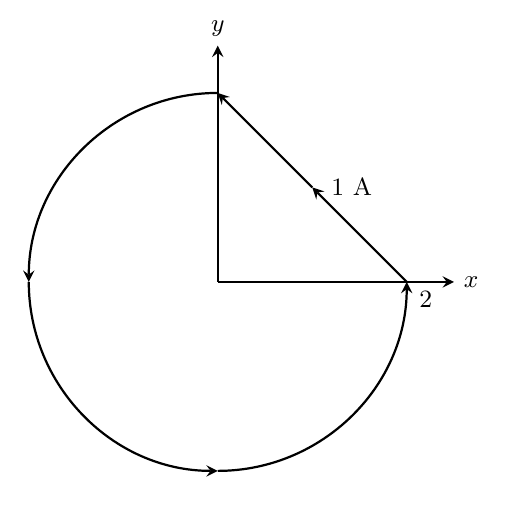
\begin{tikzpicture}[xscale=1.2,yscale=1.2,font=\small]
	\def\XD{0cm}
	\def\YD{0cm}

	\draw[thick, ->, >=stealth] (2cm, 0cm) -- (1cm, 1cm);
	\draw[thick, ->, >=stealth] (1cm, 1cm) -- (0cm, 2cm);
%	\draw[thick, ->, >=stealth] (2cm, 2cm) -- (1cm, 2cm);
%	\draw[thick, ->, >=stealth] (1cm, 2cm) -- (0cm, 2cm);
	\draw[thick, ->, >=stealth] (0,2cm)  arc (90:180:2); % -- (0cm, 0cm);
	\draw[thick, ->, >=stealth] (-2,0cm)  arc (180:270:2); % -- (0cm, 0cm);
	\draw[thick, ->, >=stealth] (0,-2cm)  arc (270:360:2); % -- (0cm, 0cm);
	%\node[above] at (0.75cm, 0.2cm){$60^0$};
	
	\coordinate[label=below:$2$] (x2) at (2.2cm,0cm);
	\coordinate[label=right:$1$ A] (1A) at (1.1cm,1cm);
	
	\draw[thick, ->, >=stealth] (0cm, 0cm) -- (0cm, 2.5cm);
	\coordinate[label=above:$y$] (y) at (0cm,2.5cm);
	\draw[thick, ->, >=stealth] (0cm, 0cm) -- (2.5cm, 0cm);
	\coordinate[label=right:$x$] (x) at (2.5cm,0cm);
\end{tikzpicture}
\end{figure}
\newpage
\noindent\textbf{Question 8: Ampere's Law \hfill \Qeight~marks}\\
Current density in a straight wire of radius 1 mm is $\textbf{J}=\dfrac{1}{2\pi}\times 10^3\hat z$ A/m$^2$. Find \textbf{H}--field everywhere.\\
\newpage
\noindent\textbf{Question 9: Electromagnetic Waves \hfill \Qnine~marks}\\
How are electromagnetic waves produced?
\newpage
\noindent\textbf{Question 10: Maxwell's Equations \hfill \Qten~marks}\\
Write Maxwell's equations in their final form.
\end{document}